\section{Finite Span Wing}
Even in inviscid flow, with no friction, there is an induced drag due to downwash generated from wing-tip vorticies. During take-off and landing, the induced drag accounts for $~60\%$ of the total drag. During cruising, it accounts for about $25\%$. There are wing-tip devices to reduce this amount of drag by reducing the vorticies.
\subsection*{Wing-tip vortex}
$\alpha_\text{eff}=\alpha-\alpha_i$\\
$\alpha_i=\tan^{-1}\left(\frac{-V_D}{V_\infty}\right)\approx-\frac{V_D}{V_\infty}$\\
$D_i'=L'\sin\alpha_i\approx L'\alpha_i$\\
$c_l=a_0\left[\alpha_\text{eff}-\alpha_{L=0}\right]=2\pi\left[\alpha-\alpha_i-\alpha_{L=0}\right]$\\
$c_l=\frac{2\Gamma}{V_\infty c}$\\
$\alpha_\text{eff}=\frac{\Gamma}{\pi V_\infty c}+\alpha_{L=0}$
\subsection*{Vortex filament (Biot-Savant's law)}
$V=\frac{\Gamma}{4\pi r}$\hfill(semi-infinite)\\
$V=\frac{\Gamma}{2\pi r}$\hfill(infinitely long)
\subsection*{Prandtl's lifting line theorem}
$V_D=-\frac{1}{4\pi}\intoverspan\frac{\left(\odv{\Gamma}/{\zeta}\right)\odif{\zeta}}{z-\zeta}$\\
$\alpha_i=-\frac{V_D}{V_\infty}=\frac{1}{4\pi V_\infty}\intoverspan\frac{\left(\odv{\Gamma}/{\zeta}\right)\odif{\zeta}}{z-\zeta}$\\
$\alpha=\frac{\Gamma}{\pi V_\infty c}+\alpha_{L=0}+\frac{1}{4\pi V_\infty}\intoverspan\frac{\left(\odv{\Gamma}/{\zeta}\right)\odif{\zeta}}{z-\zeta}$
\subsection*{2D vs. 3D definitions}
% $L'(z)=\rho V_\infty \Gamma(z)$\\
$L=\intoverspan L'(z)\odif{z}=\rho V_\infty\intoverspan \Gamma(z)\odif{z}$\\
% $C_{L,\text{3D}}=\frac{L_\text{3D}}{\sfrac{1}{2}\rho V_\infty^2 S}$\hfill\text{(3D lift coefficient)}\\
$C_L=\frac{2}{V_\infty S}\intoverspan\Gamma(z)\odif{z}$\\
$D_i=\intoverspan L'(z)\alpha_i\odif{z}=\rho V_\infty\intoverspan \Gamma(z)\alpha_i\odif{z}$\\
$C_{D,i}=\frac{2}{V_\infty S}\intoverspan \Gamma(z)\alpha_i\odif{z}$
\subsection*{Elliptic distribtion assumption}
$\Gamma(z)=\Gamma_o\sqrt{1-\left(\frac{2z}{b}\right)^2}$\hfill\text{(assume true)}\\
$V_D=-\frac{\Gamma_o}{2b}$\\
$L=\rho V_\infty\Gamma_o\frac{\pi b}{4}$\\
$C_L=\frac{\Gamma_o\pi b}{2V_\infty S}$\\
$\AR\defequals\frac{b^2}{S}$\hfill(aspect ratio, span$^2$:area)\\
$\alpha_i=\frac{\Gamma_o}{2bV_\infty}=\frac{SC_L}{\pi b^2}=\frac{C_L}{\pi \AR}$\\
$C_{D,i}=\frac{\pi\alpha_i\Gamma_0 b}{2V_\infty S}=\frac{C_L^2}{\pi\AR}$\\
$l(z)=\frac{2\Gamma(z)}{V_\infty C_L}$\\
$a\defequals\odv*[fun=true]{C_L}{\alpha}$\hfill(slope of 3D lift curve)\\
$a=\frac{a_o}{1+\frac{a_o}{\pi\AR}}$\\
Elliptic planform gives the minimum induced drag.\\
\subsection*{Non-elliptic planform}
$\Gamma(\theta)=2bV_\infty\sum_{n=1}^NA_n\sin\left(n\theta\right)$\\
$L=\frac{\pi\rho V_\infty^2 b^2 A_1}{2}$\\
$C_L=\frac{L}{\sfrac{1}{2}\rho V_\infty^2 S}=A_1\pi\frac{b^2}{S}=A_1\pi\AR $\\
$\alpha_i=\frac{1}{4\pi V_\infty}\intoverspan\frac{\left(\odv{\Gamma}/{\zeta}\right)\odif{\zeta}}{z-\zeta}$\\
$C_{D,i}=\frac{C_L^2}{\pi\AR}\left[1+\sum_{n=2}^Nn\left(\frac{A_n}{A_1}\right)^2\right]$\\
$\epsilon_1\defequals\sum_{n=2}^Nn\left(\frac{A_n}{A_1}\right)^2$\\
$C_{D,i}=\frac{C_L^2}{\pi\AR}\left(1+\epsilon_1\right)$\\
$C_{D,i}\propto C_L^2\propto \sfrac{1}{\AR}$\\
$a=\frac{a_o}{1+\frac{a_o(1+\epsilon_2)}{\pi\AR}}$\hfill(reduced WRT elliptic)\\
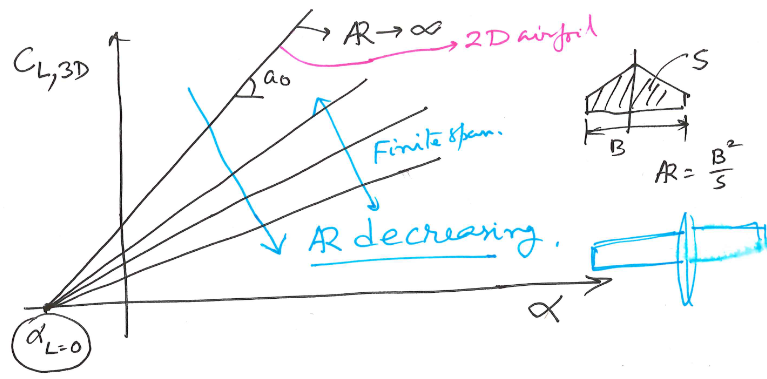
\includegraphics[width=140pt]{images/aspect affect cl.png}

